\section{ИССЛЕДОВАНИЕ РАБОТЫ СУММАТОРА}

\begin{figure}[H]
	\centering
	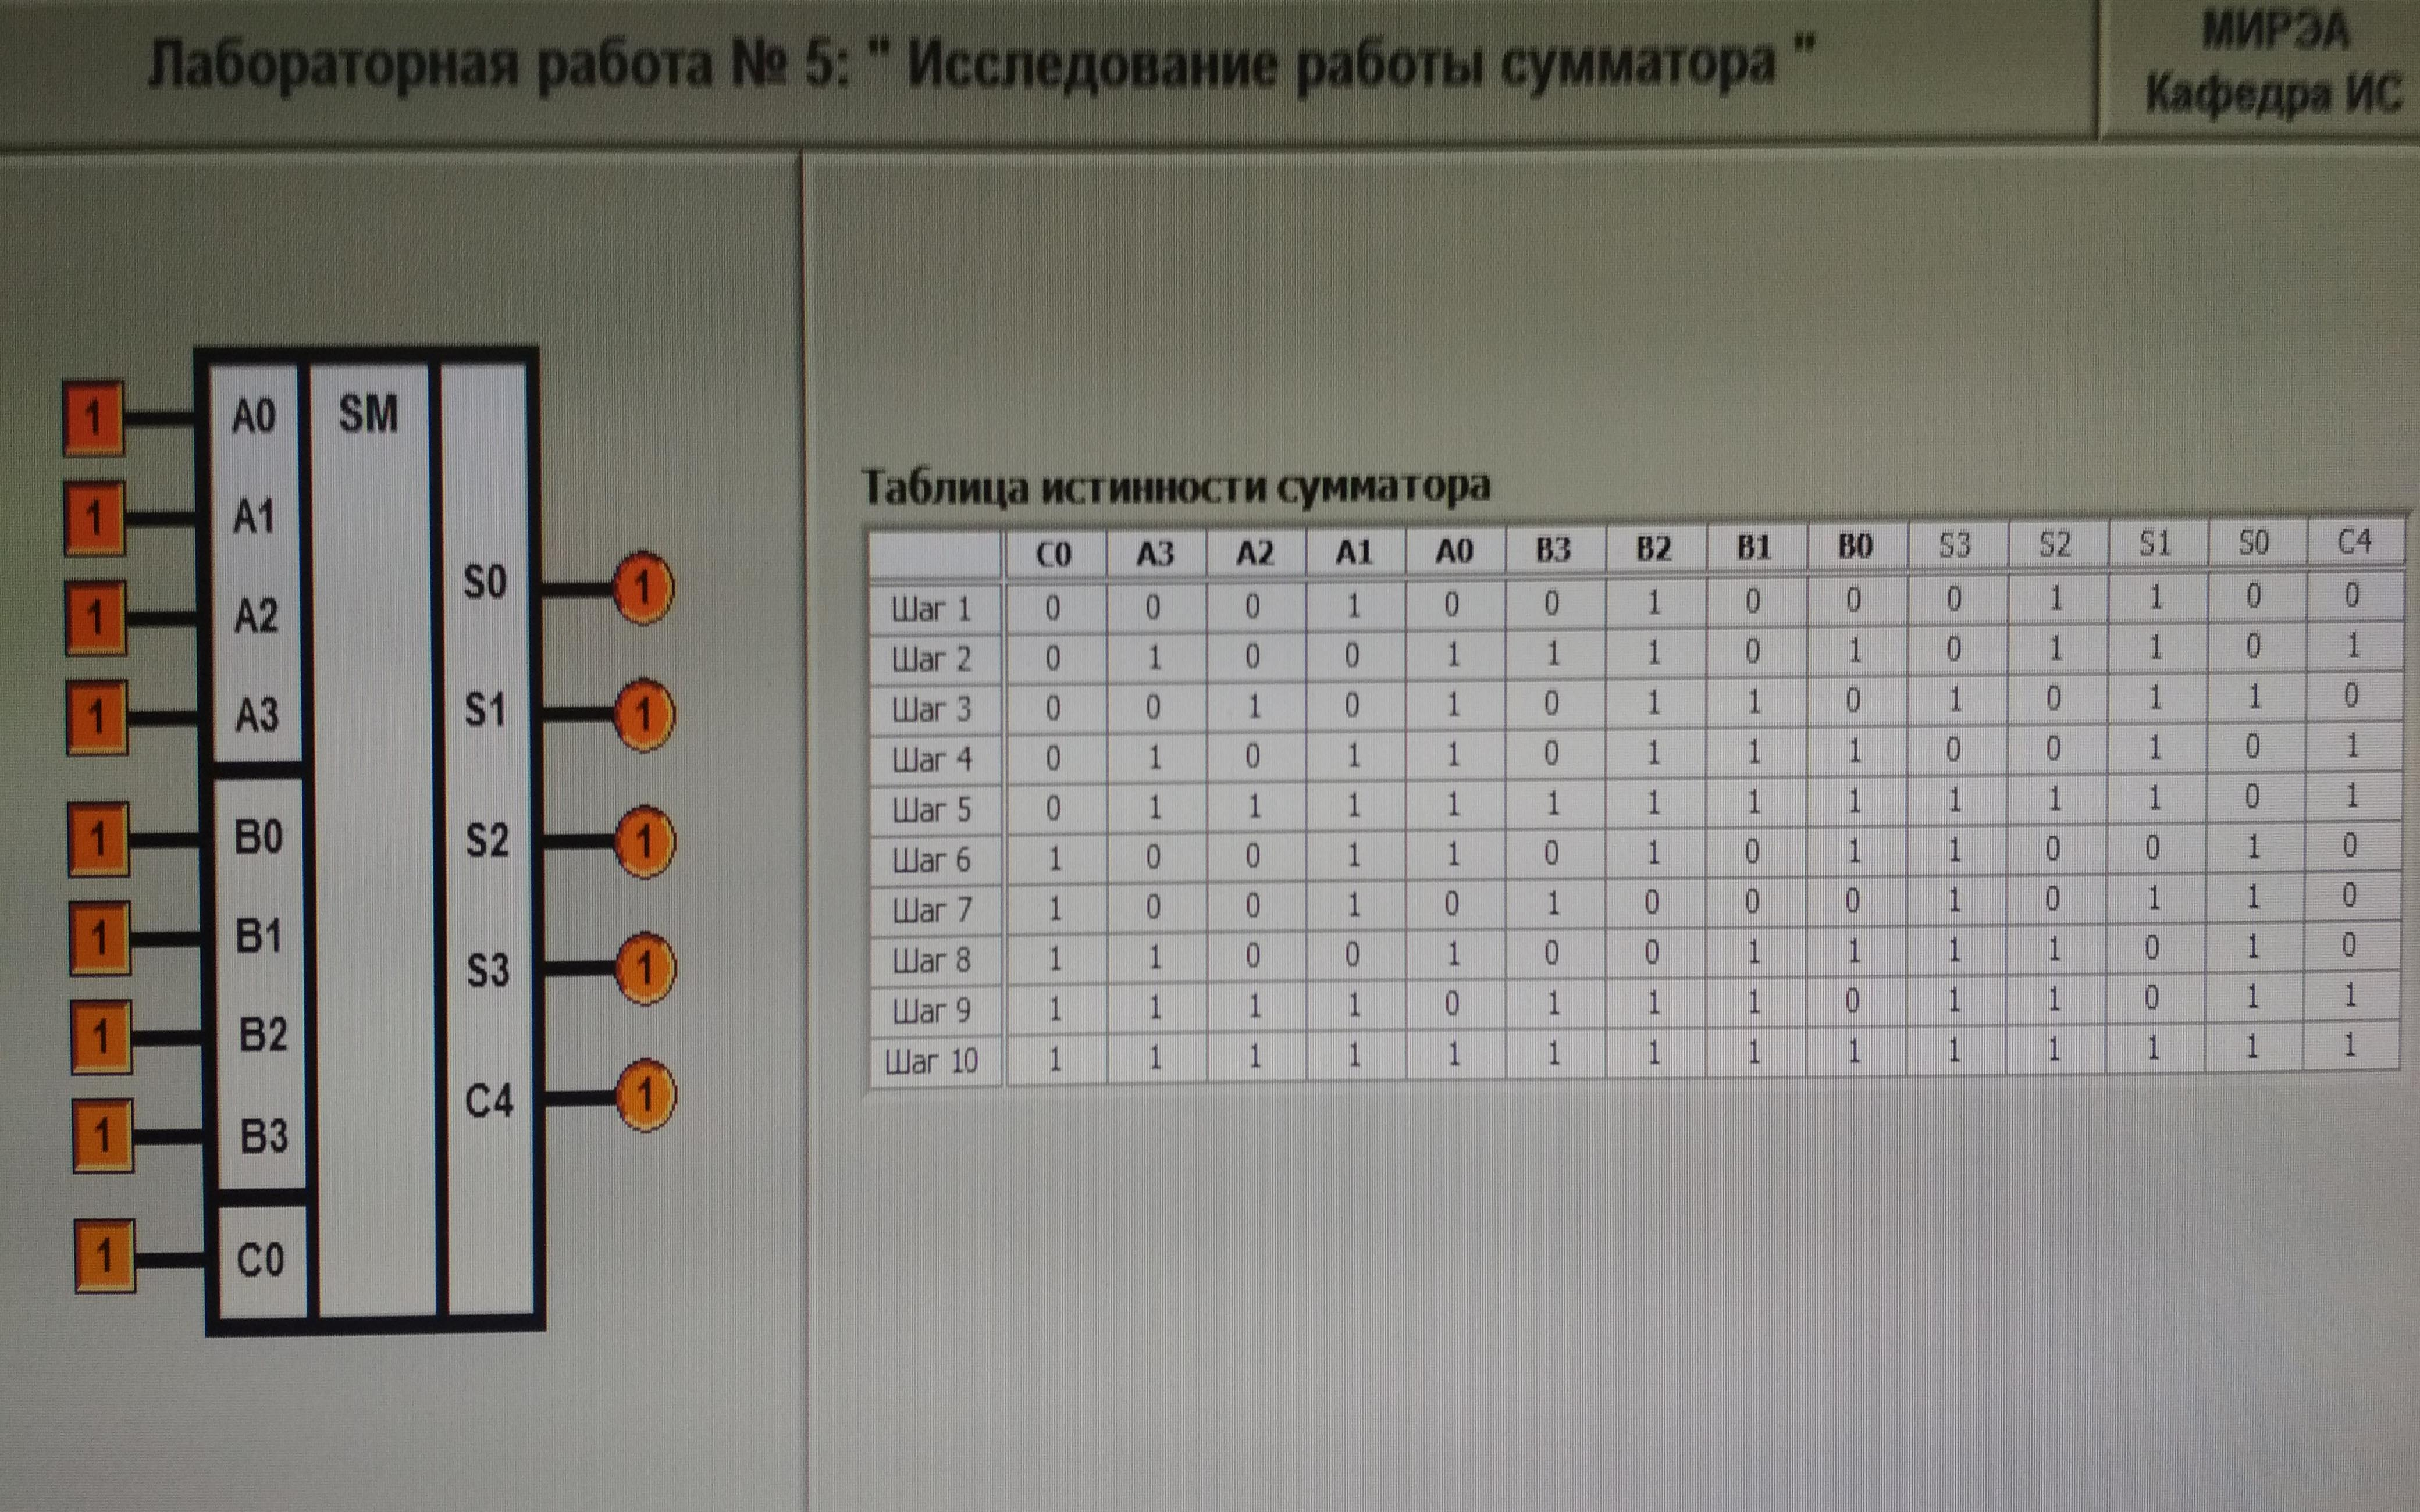
\includegraphics[width=0.95\linewidth]{imgs/5/1}
	\caption{Результат работы сумматора}
	\label{fig:5_}
\end{figure}

\begin{table}[H]
	\centering
	\caption{Проверка работы сумматора}
	\label{tab:lab_05}
	\begin{tabular}{|c|c|c|c|c|c|c|c|c|c|c|c|c|c|c|c|c|}
		\hline
		C0 & A3 & A2 & A1 & A0 & B3 & B2 & B1 & B0 &    & S3 & S2 & S1 & S0 & C4 &    &      \\ \hline
		0  & 0  & 0  & 1  & 0  & 0  & 1  & 0  & 0  & 6  & 0  & 1  & 1  & 0  & 0  & 6  & TRUE \\ \hline
		0  & 1  & 0  & 0  & 1  & 1  & 1  & 0  & 1  & 22 & 0  & 1  & 1  & 0  & 1  & 22 & TRUE \\ \hline
		0  & 0  & 1  & 0  & 1  & 0  & 1  & 1  & 0  & 11 & 1  & 0  & 1  & 1  & 0  & 11 & TRUE \\ \hline
		0  & 1  & 0  & 1  & 1  & 0  & 1  & 1  & 1  & 18 & 0  & 0  & 1  & 0  & 1  & 18 & TRUE \\ \hline
		0  & 1  & 1  & 1  & 1  & 1  & 1  & 1  & 1  & 30 & 1  & 1  & 1  & 0  & 1  & 30 & TRUE \\ \hline
		1  & 0  & 0  & 1  & 1  & 0  & 1  & 0  & 1  & 9  & 1  & 0  & 0  & 1  & 0  & 9  & TRUE \\ \hline
		1  & 0  & 0  & 1  & 0  & 1  & 0  & 0  & 0  & 11 & 1  & 0  & 1  & 1  & 0  & 11 & TRUE \\ \hline
		1  & 1  & 0  & 0  & 1  & 0  & 0  & 1  & 1  & 13 & 1  & 1  & 0  & 1  & 0  & 13 & TRUE \\ \hline
		1  & 1  & 1  & 1  & 0  & 1  & 1  & 1  & 0  & 29 & 1  & 1  & 0  & 1  & 1  & 29 & TRUE \\ \hline
		1  & 1  & 1  & 1  & 1  & 1  & 1  & 1  & 1  & 31 & 1  & 1  & 1  & 1  & 1  & 31 & TRUE \\ \hline
	\end{tabular}
\end{table}

Элемент CD5474ACT283 - Advanced CMOS

Характеристики:

\begin{figure}[H]
	\centering
	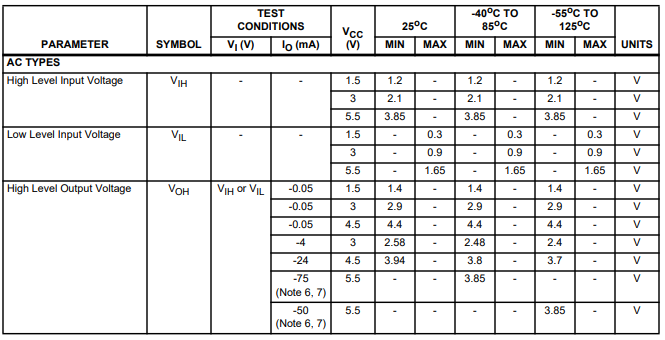
\includegraphics[width=0.95\linewidth]{imgs/5/ti1}
	\caption{Электрические парамеры}
	\label{fig:5_ti1}
\end{figure}

\begin{figure}[H]
	\centering
	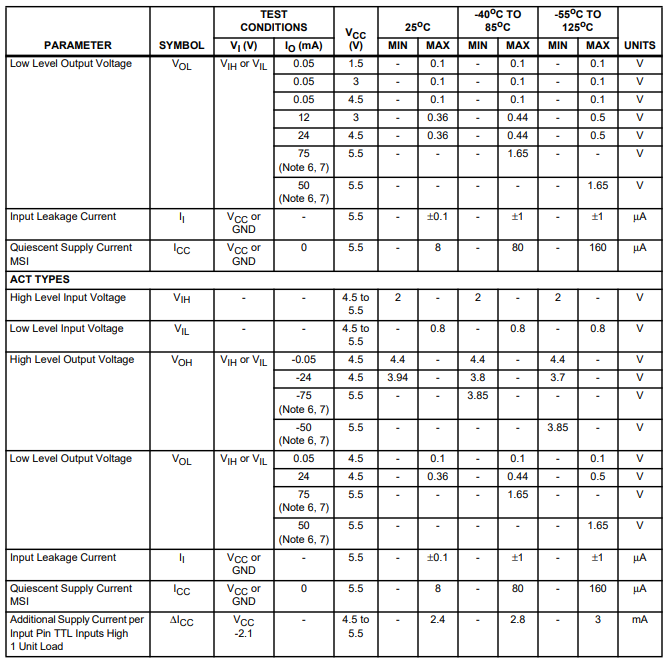
\includegraphics[width=0.95\linewidth]{imgs/5/ti2}
	\caption{Электрические парамеры}
	\label{fig:5_ti2}
\end{figure}

\begin{figure}[H]
	\centering
	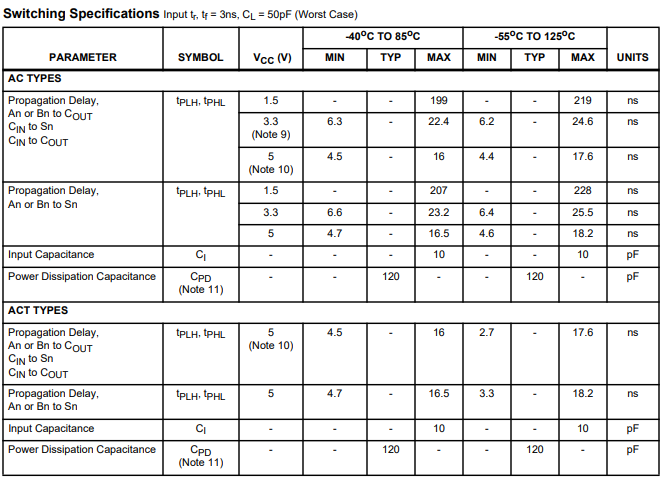
\includegraphics[width=0.95\linewidth]{imgs/5/ti3}
	\caption{Параметры переключения}
	\label{fig:5_ti3}
\end{figure}
